\documentclass[letterpaper,11pt,leqno]{article}
\usepackage{paper}
\usepackage{natbib}
\bibliographystyle{bibliography}

\usepackage{xcolor}
\usepackage{hyperref}
\usepackage{threeparttable}
\usepackage{natbib}
\usepackage{listings}
\usepackage{rotating}
\usepackage{float}
\usepackage{pdflscape}
\usepackage{makecell}
\usepackage{booktabs}

\definecolor{customblue}{rgb}{0,0.337,0.702}

\hypersetup{
    colorlinks   = true,
    citecolor    = customblue,
    linkcolor    = customblue,
    urlcolor     = customblue
}

\newenvironment{fignotes}{\setstretch{1.2}\scriptsize}

\newenvironment{fignotes2}{\begin{quote}\setstretch{1.2}\scriptsize}{\end{quote}}

\def\dotfill#1{\cleaders\hbox to #1{.}\hfill}
\makeatletter
\def\myrulefill{\leavevmode\leaders\hrule height .7ex width 1ex depth -0.6ex\hfill\kern\z@}
\makeatother

\begin{document}

\title{\Large \textsc{A simple and adaptable method to estimate the income distribution in Spain}}

\author{\href{https://pablogguz.github.io/}{\large{Pablo García-Guzmán}\thanks{Email: \href{mailto:pablo.garcia-guzman@ebrd.com}{garciagp@ebrd.com}. I thank Pedro Torres for his valuable feedback and comments. The views expressed in this methodology note are completely my own and do not reflect the views of the EBRD.}} \\ \normalsize{EBRD}}

\date{\normalsize \today \\}

% \textcolor{red}{Preliminary draft -- do not cite or circulate}

\maketitle
\begin{abstract}
\onehalfspacing
This methodology note develops a transparent and simple framework to estimate aggregate income distributions in Spain exploiting the availability of granular inequality metrics. Specifically, I leverage administrative tax records and demographic data at the census tract-level to reconstruct local income distributions assuming log-normality. National, regional and municipal income distributions can be subsequently derived as population-weighted mixtures of these tract-level distributions. This approach leverages well-documented regularities in how incomes are distributed within demographically homogeneous groups, and the resulting estimates closely match observed distributional statistics in validation tests. I implement this framework in \href{https://comparatuingreso.es/}{comparatuingreso.es}, a publicly available web platform that enables Spanish households to calculate their relative position within the income distribution. While the focus is on Spain, this approach can be readily adapted to other countries with comparable data available.
\end{abstract}

\thispagestyle{empty}

\newpage

\setcounter{page}{1}

\section{Introduction}

Understanding the income distribution is crucial for economic analysis and policy design, yet its measurement remains challenging. In this paper, I propose a transparent and simple method to estimate national-level income distributions when granular income and inequality measures are available. The approach builds on two key insights: first, that income distributions within demographically homogeneous areas tend to follow log-normal distributions; and second, that aggregate distributions can be effectively modeled as mixtures of these local distributions. Using detailed administrative data from over 36,000 Spanish census tracts, I demonstrate that local income distributions are well-approximated by log-normal distributions, with predicted statistics matching observed values within 5\% on average. This method provides a flexible parametric framework for estimating income distributions when individual data is unavailable

%Using detailed administrative data from Spain covering over 36,000 census tracts, I show that local income distributions are well-approximated by log-normal distributions, with predicted statistics matching observed values within 5\% on average. This sets the ground for estimating aggregate income distribution as a population-weighted mixture of tract-specific log-normals. The method provides a flexible framework for estimating income distributions when individual data is unavailable.

The rest of this note is organized as follows. Section \ref{sec:data} describes the data sources, their coverage, and scope. Section \ref{sec:method} outlines the methodology, including the modeling of local income distributions, their aggregation and the calculation of the relevant validation metrics. Section \ref{sec:results} presents the results. Finally, Section \ref{sec:conc} concludes the note.

\section{Data}\label{sec:data}


The data used in this project is sourced from the Spanish Statistical Office (INE) Household Income Distribution Atlas (\textit{Atlas de Distribución de Renta de los Hogares}, ADRH). This dataset combines administrative tax data with population statistics to provide detailed information about the income distribution and related socioeconomic indicators at granular geographic levels in Spain.

Spain is administratively divided into several territorial levels that structure its governance and statistical reporting. At the highest level are the \textit{Comunidades Autónomas} (Autonomous Communities), which are regions with significant legislative and executive powers granted by the Spanish Constitution. There are 17 Autonomous Communities and two Autonomous Cities (Ceuta and Melilla). These regions are further subdivided into \textit{provincias} (provinces), the primary intermediate level of governance. Each province consists of \textit{municipios} (municipalities), the fundamental local administrative units, which vary widely in size and population.

Below the municipal level, finer geographic divisions provide additional granularity. Larger municipalities are typically divided into \textit{distritos} (districts), which correspond to distinct urban or rural areas within the municipality. The smallest unit of analysis is the \textit{sección censal} (census tract), encompassing areas with populations ranging from 1,000 to 2,500 residents. Census tracts provide the finest level of geographic detail available in the ADRH.

Income data in the ADRH is derived from tax declarations submitted to the Spanish tax authorities, including the \textit{Agencia Estatal de Administración Tributaria} (AEAT) and the Foral tax authorities.\footnote{The latter operate in regions with special fiscal regimes, such as the Basque Country and Navarre.} These tax records provide detailed information on income from various sources, including wages, pensions, unemployment benefits, and other forms of revenue subject to the \text{Impuesto sobre la Renta de las Personas Físicas} (IRPF), Spain's personal income tax system. The dataset excludes non-resident income and focuses exclusively on individuals considered fiscal residents within the territory.

Demographic data in the ADRH is constructed from the \textit{Fichero Precensal de Población} (FPC), a comprehensive register derived from the municipal register (\textit{Padrón}) and other administrative sources. The FPC forms the basis of Spain’s population census and ensures alignment between demographic and income data. The temporal reference for income data corresponds to the calendar year, while demographic data is anchored to the population as registered on January 1 of the following year. Individuals residing in collective establishments, such as nursing homes, hospitals, or military barracks, are excluded from the dataset.

\paragraph{Summary statisticts}.


\begin{table}[H]
\centering
\resizebox{0.8\textwidth}{!}{% 
\begin{threeparttable}[H]
\onehalfspacing
\centering
\captionsetup{justification=centering} 
\caption{Covid impact}

\begin{tabular}{@{}lccccc@{}}
\toprule
  & (1) & (2) & (3) &  (4) &  (5) \\
 & Min & Max & Mean & SD & \% missing\\
\midrule
\qquad \textit{Income distribution} \\
Net income per capita &  4,996.00 & 34,765.00 & 14,030.16 &  4,193.34 &      1.63\\
Net income per equivalent adult &  8,092.00 & 55,987.00 & 20,797.51 &  6,628.08 &      5.20\\
Gini &     20.30 &     44.20 &     29.02 &      3.84 &      5.20\\
\qquad \textit{Demographics} \\
Population &      3.00 & 12,144.00 &  1,303.10 &    663.26 &      1.45\\
Dependency ratio &      0.09 &      4.00 &      0.63 &      0.17 &      1.45\\
Mean age &     27.40 &     74.70 &     45.43 &      5.52 &      1.45\\
Single-person households (%) &      0.00 &    100.00 &     30.50 &      9.56 &      1.45\\
\midrule
No. of tracts &          36,982 \\
\midrule
\end{tabular}
\begin{tablenotes}[para,flushleft]
\footnotesize 
\textbf{Source}: Spanish Statistical Office (INE) Household Income Distribution Atlas and author's calculations.
\end{tablenotes}
\end{threeparttable}
}
\end{table}

\section{Methodology}\label{sec:method}


\subsection{Background}

The study of income distributions has been a cornerstone of economic research. A long-standing empirical regularity in the literature is that income distributions tend to approximate log-normality \citep{aitchison1957lognormal}. This stylized fact is supported by theoretical and empirical foundations. At its core, log-normality arises from the multiplicative interaction of economic factors—such as human capital, local labor market conditions, and productivity—which determine individual incomes \citep{neal2000theories}. Gibrat's Law of Proportionate Effect \citep{gibrat1931inegalites} formalizes a theoretical foundation for log-normality through multiplicative random growth, showing that when the growth rate of a variable is independent of its initial size and the logarithm of the growth rate is independent and identically distributed over time with finite variance, the resulting distribution tends to converge to log-normality. Empirically, log-normal densities have been shown to approximate very well per capita income distributions in large cross-country panels \citep{lopez2006normal}.

More concretely, the multiplicative processes through which log-normality arises operate most strongly within demographically homogeneous groups where individuals are subject to similar economic shocks \citep{battistin2009consumption}. The literature of neighborhood effects offers a complementary explanation for why such homogeneity in income-generating processes exists at local levels. Specifically, neighborhood effects reinforce homogeneity within local populations through contextual influences (e.g., average neighborhood income or quality of local services) and endogenous spillovers, which emerge from behavioral interactions within the neighborhood, such as peer influences or social norms \citep{manski1993identification, durlauf1996neighborhoods}. These mechanisms create reinforcing feedback loops that generate correlated income trajectories within neighborhoods -- for instance, through shared information about job opportunities, similar human capital accumulation patterns, or common responses to local economic shocks.  The resulting interaction structures generate strong within-neighborhood homogeneity while maintaining between-neighborhood heterogeneity \citep{durlauf2004neighborhood}. This pattern provides a theoretical rationale  for estimating aggregate income distributions as mixtures of local-level distributions.

%Relatedly, a more recent literature on place effects has documented that the environment where children grow up has substantial causal impacts on their economic outcomes later in life \cite{chynplace}. Using experimental variation from the Moving to Opportunity program, \cite{chetty2016effects} show that childhood exposure to better neighborhoods significantly increases college attendance and earnings in adulthood.

The log-normal distribution, while providing a good approximation for much of the income distribution, exhibits systematic deviations in the tails. Since Pareto's \citeyearpar{pareto1896cours} original work, research has shown that top incomes follow a power law rather than a log-normal decay \citep{gabaix2016power}. Similarly, studies using detailed administrative tax data have documented that the upper tail of income distributions across countries and time periods are better described by a Pareto distribution \citep{atkinson2011top}. This departure from log-normality at high incomes is important for accurately measuring top income inequality, but modeling the precise behavior of the upper tail is beyond the scope of this note.

\subsection{Empirical approach}

I estimate the national income distribution by exploiting the granular structure of census tract data and the theoretical properties of income distributions. My approach leverages two key insights: (1) income distributions within small geographic units tend to follow log-normal distributions more closely than in larger areas, and (2) the overall distribution can be approximated by a mixture of these local distributions.

Consider a census tract $j$ with an observed mean income $\mu_j$ and Gini coefficient $G_j$. Under the log-normality assumption, if income $Y$ follows a log-normal distribution with parameters $(\nu_j, \sigma_j^2)$, then:

\begin{equation}
\ln(Y) \sim N(\nu_j, \sigma_j^2)
\end{equation}

The relationship between these parameters and the observed statistics is thus given by:

\begin{equation}
\mu_j = \exp\left(\nu_j + \frac{\sigma_j^2}{2}\right)
\end{equation}

\begin{equation}
G_j = 2\Phi\left(\frac{\sigma_j}{\sqrt{2}}\right) - 1
\end{equation}

where $\Phi(\cdot)$ is the standard normal cumulative distribution function. From the observed Gini coefficient, I can recover $\sigma_j$:

\begin{equation}
\sigma_j = \sqrt{2}\Phi^{-1}\left(\frac{G_j + 1}{2}\right)
\end{equation}

Given $\sigma_j$ and $\mu_j$, the distribution for census tract $j$ is fully identified, , as $\nu_j$ can be solved analytically. I then estimate the national distribution as a population-weighted mixture of these local log-normal distributions. For a given income level $y$, the density is given by:

\begin{equation}
f(y) = \sum_{j=1}^{J} w_j f_j(x|\nu_j,\sigma_j^2)
\end{equation}

where $w_j$ is tract $j$'s population share and $f_j(\cdot|\nu_j,\sigma_j^2)$ is the log-normal density function with parameters $(\nu_j,\sigma_j^2)$.

To calculate percentiles of the national distribution, I solve:

\begin{equation}
p = F(q_p) = \sum_{j=1}^{J} w_j \Phi\left(\frac{\ln(q_p) - \nu_j}{\sigma_j}\right)
\end{equation}

where $q_p$ is the $p^{th}$ percentile and $F(\cdot)$ is the cumulative distribution function of the mixture. I use numerical root-finding methods to find the value of $q_p$ that satisfies $F(q_p) - p = 0$ within a bounded interval.

This approach has several advantages. First, it respects the theoretical properties of income distributions at local levels where populations are relatively homogeneous. Second, it preserves tract-level moments while allowing for heterogeneity across tracts. Third, it provides a flexible framework that can be adapted and extended to calculate any distributional statistic of interest.

\paragraph{Missing outcomes} For census tracts with missing Gini coefficients (approximately 5.2\% of the sample), I estimate them using machine learning methods. Specifically, I train an XGBoost model using the following demographic predictors: dependency ratio (ratio of population under 18 and over 65 to working-age population), mean age, percentage of single-person households, mean logged equivalised income, and province fixed effects. Model performance is validated using a 5-fold cross-validation procedure. The XGBoost model is trained using default hyperparameters without grid search or additional tuning. Results are shown in Table \ref{perf}. Based on the cross-validation results, the XGBoost model demonstrates superior predictive performance compared to a baseline OLS model, as illustrated by a 11\% lower RMSE.

\begin{table}[H]
\centering
\resizebox{0.7\textwidth}{!}{% 
\begin{threeparttable}[H]
\onehalfspacing
\centering
\captionsetup{justification=centering} 
\caption{Performance comparison between OLS and XGBoost models}\label{perf}
\begin{tabular}{lccc}
\hline
Model    & RMSE & MAE & MAPE (\%) \\
\hline
OLS                & 3.15          & 2.41         & 8.32              \\
XGBoost (CV)       & 2.81          & 2.17         & 7.49              \\
\hline
Relative improvement over OLS (\%) & 10.8\% & 10.0\% & 10.0\% \\
\hline
\end{tabular}
\begin{tablenotes}[para,flushleft]
\scriptsize 
\textbf{Notes}: This table compares the performance of two predictive models—OLS and XGBoost—on predicting missing Gini coefficients using demographic predictors. RMSE represents the root mean square error, MAE is the mean absolute error, and MAPE is the mean absolute percentage error. Relative improvements in each metric are calculated as the percentage reduction of the error metric when using XGBoost compared to OLS. Results are based on a 5-fold cross-validation procedure for the XGBoost model.
\end{tablenotes}
\end{threeparttable}
}
\end{table}


\paragraph{Validation} To validate the log-normality assumption at the tract level, I compare observed distributional statistics with their theoretical counterparts under log-normality. For each tract $j$, I first recover the parameters of the theoretical log-normal distribution $(\nu_j, \sigma_j)$ using the observed mean income and Gini coefficient. Then, I calculate two key predicted statistics: the P80/P20 ratio and the median income. Under log-normality, these are given by:

\begin{equation}
\text{P80/P20}_j = \exp(\sigma_j(\Phi^{-1}(0.8) - \Phi^{-1}(0.2)))
\end{equation}

\begin{equation}
\text{P50}_j = \exp(\nu_j)
\end{equation}

To assess the fit, I estimate OLS regressions of the form:

\begin{equation}
\hat{y}_j = \alpha + \beta y_j + \epsilon_j
\end{equation}

where $\hat{y}_j$ is the predicted value under log-normality and $y_j$ is the observed value.

\section{Results}\label{sec:results}


I begin by validating the log-normality assumption at the tract level. Figure \ref{fig:median} examines the fit for median income, comparing observed values with those predicted under log-normality for each census tract, where observations are grouped into equal-sized bins using binscatter methods.\footnote{See \cite{cattaneo}.} The relationship is remarkably strong ($\beta$ = 0.98, $R^2$ = 0.98), with predicted values differing from observed ones by just 4.6\% on average. The near-unit slope coefficient and $R^2$ indicate that log-normality captures the central tendency of the income distribution particularly well.

Figure \ref{fig:median} shows the relationship for the P80/P20 ratio. The regression yields a slope coefficient of 0.75 ($R^2$ = 0.81), with predicted values deviating from observed ones by 5\% on average. Consistent with the fact that real income distributions tend to have heavier tails, the coefficient below unity suggests that the log-normal distribution slightly underestimates inequality.

%Next, I show how the mixture approach generates substantial differences between the distribution implied solely by tract means -- where everyone within a tract is assumed to have the same income -- and the estimated individual-level distribution. Figure \ref{fig:distributions} plots both distributions for net equivalised income in 2022. The tract-level distribution (in dark blue) exhibits higher kurtosis and is more concentrated around its mode of approximately €20,000, as it collapses all within-tract variation to a single point. In contrast, the estimated individual distribution shows greater dispersion and a lower mode, reflecting the within-tract inequality captured by the mixture of log-normal local distributions. The heavier left tail and more gradual right tail of the mixture distribution suggest that a simple aggregation of tract means would vastly understate income inequality, particularly by failing to account for the substantial mass of low-income households and the long right tail of high earners.

\begin{figure}[H]
\begin{center}
\captionsetup{justification=centering}
\caption{Validation of log-normality: median income}
\label{fig:median}
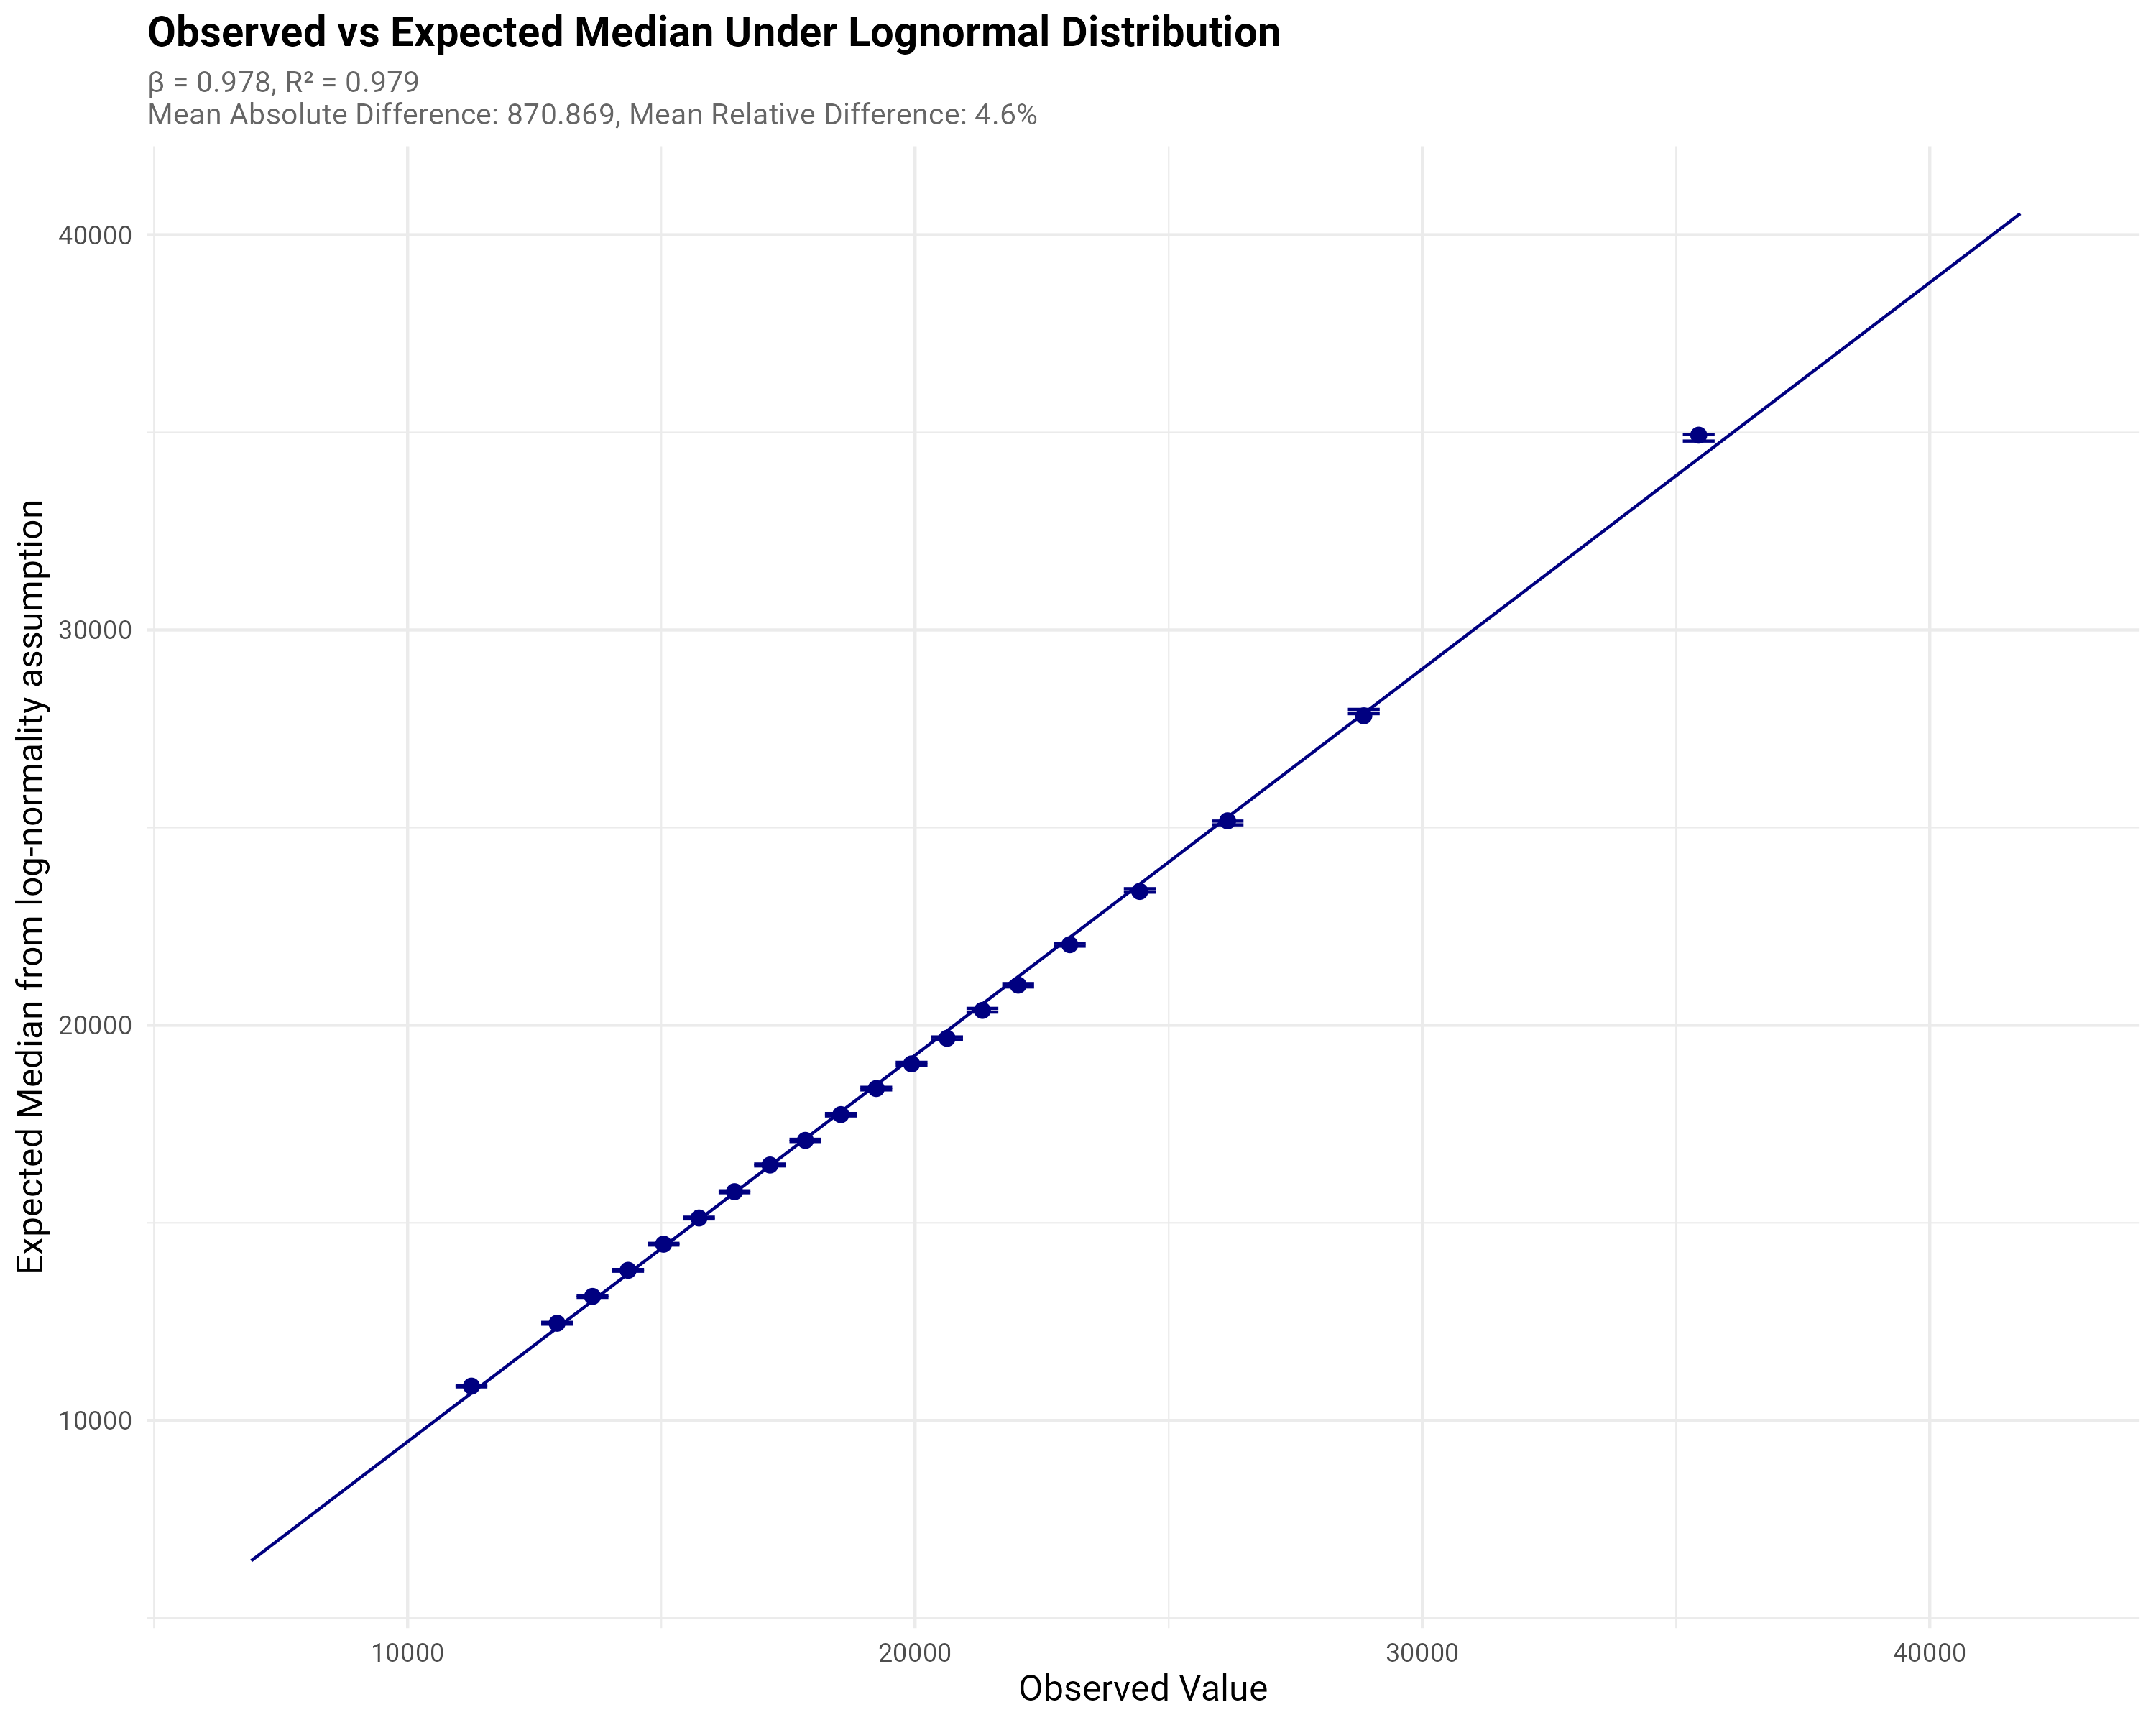
\includegraphics[width=0.85\textwidth]{output/binned_scatter_median.png}
\end{center}
\begin{fignotes2}
\textbf{Notes:} This figure shows a binned scatter plot comparing observed median income with predicted values under the log-normal assumption for each census tract. Source: Spanish Statistical Office and author's calculations.
\end{fignotes2}
\end{figure}

\begin{figure}[H]
\begin{center}
\captionsetup{justification=centering}
\caption{Validation of log-normality: P80/P20 ratio}
\label{fig:p80p20}
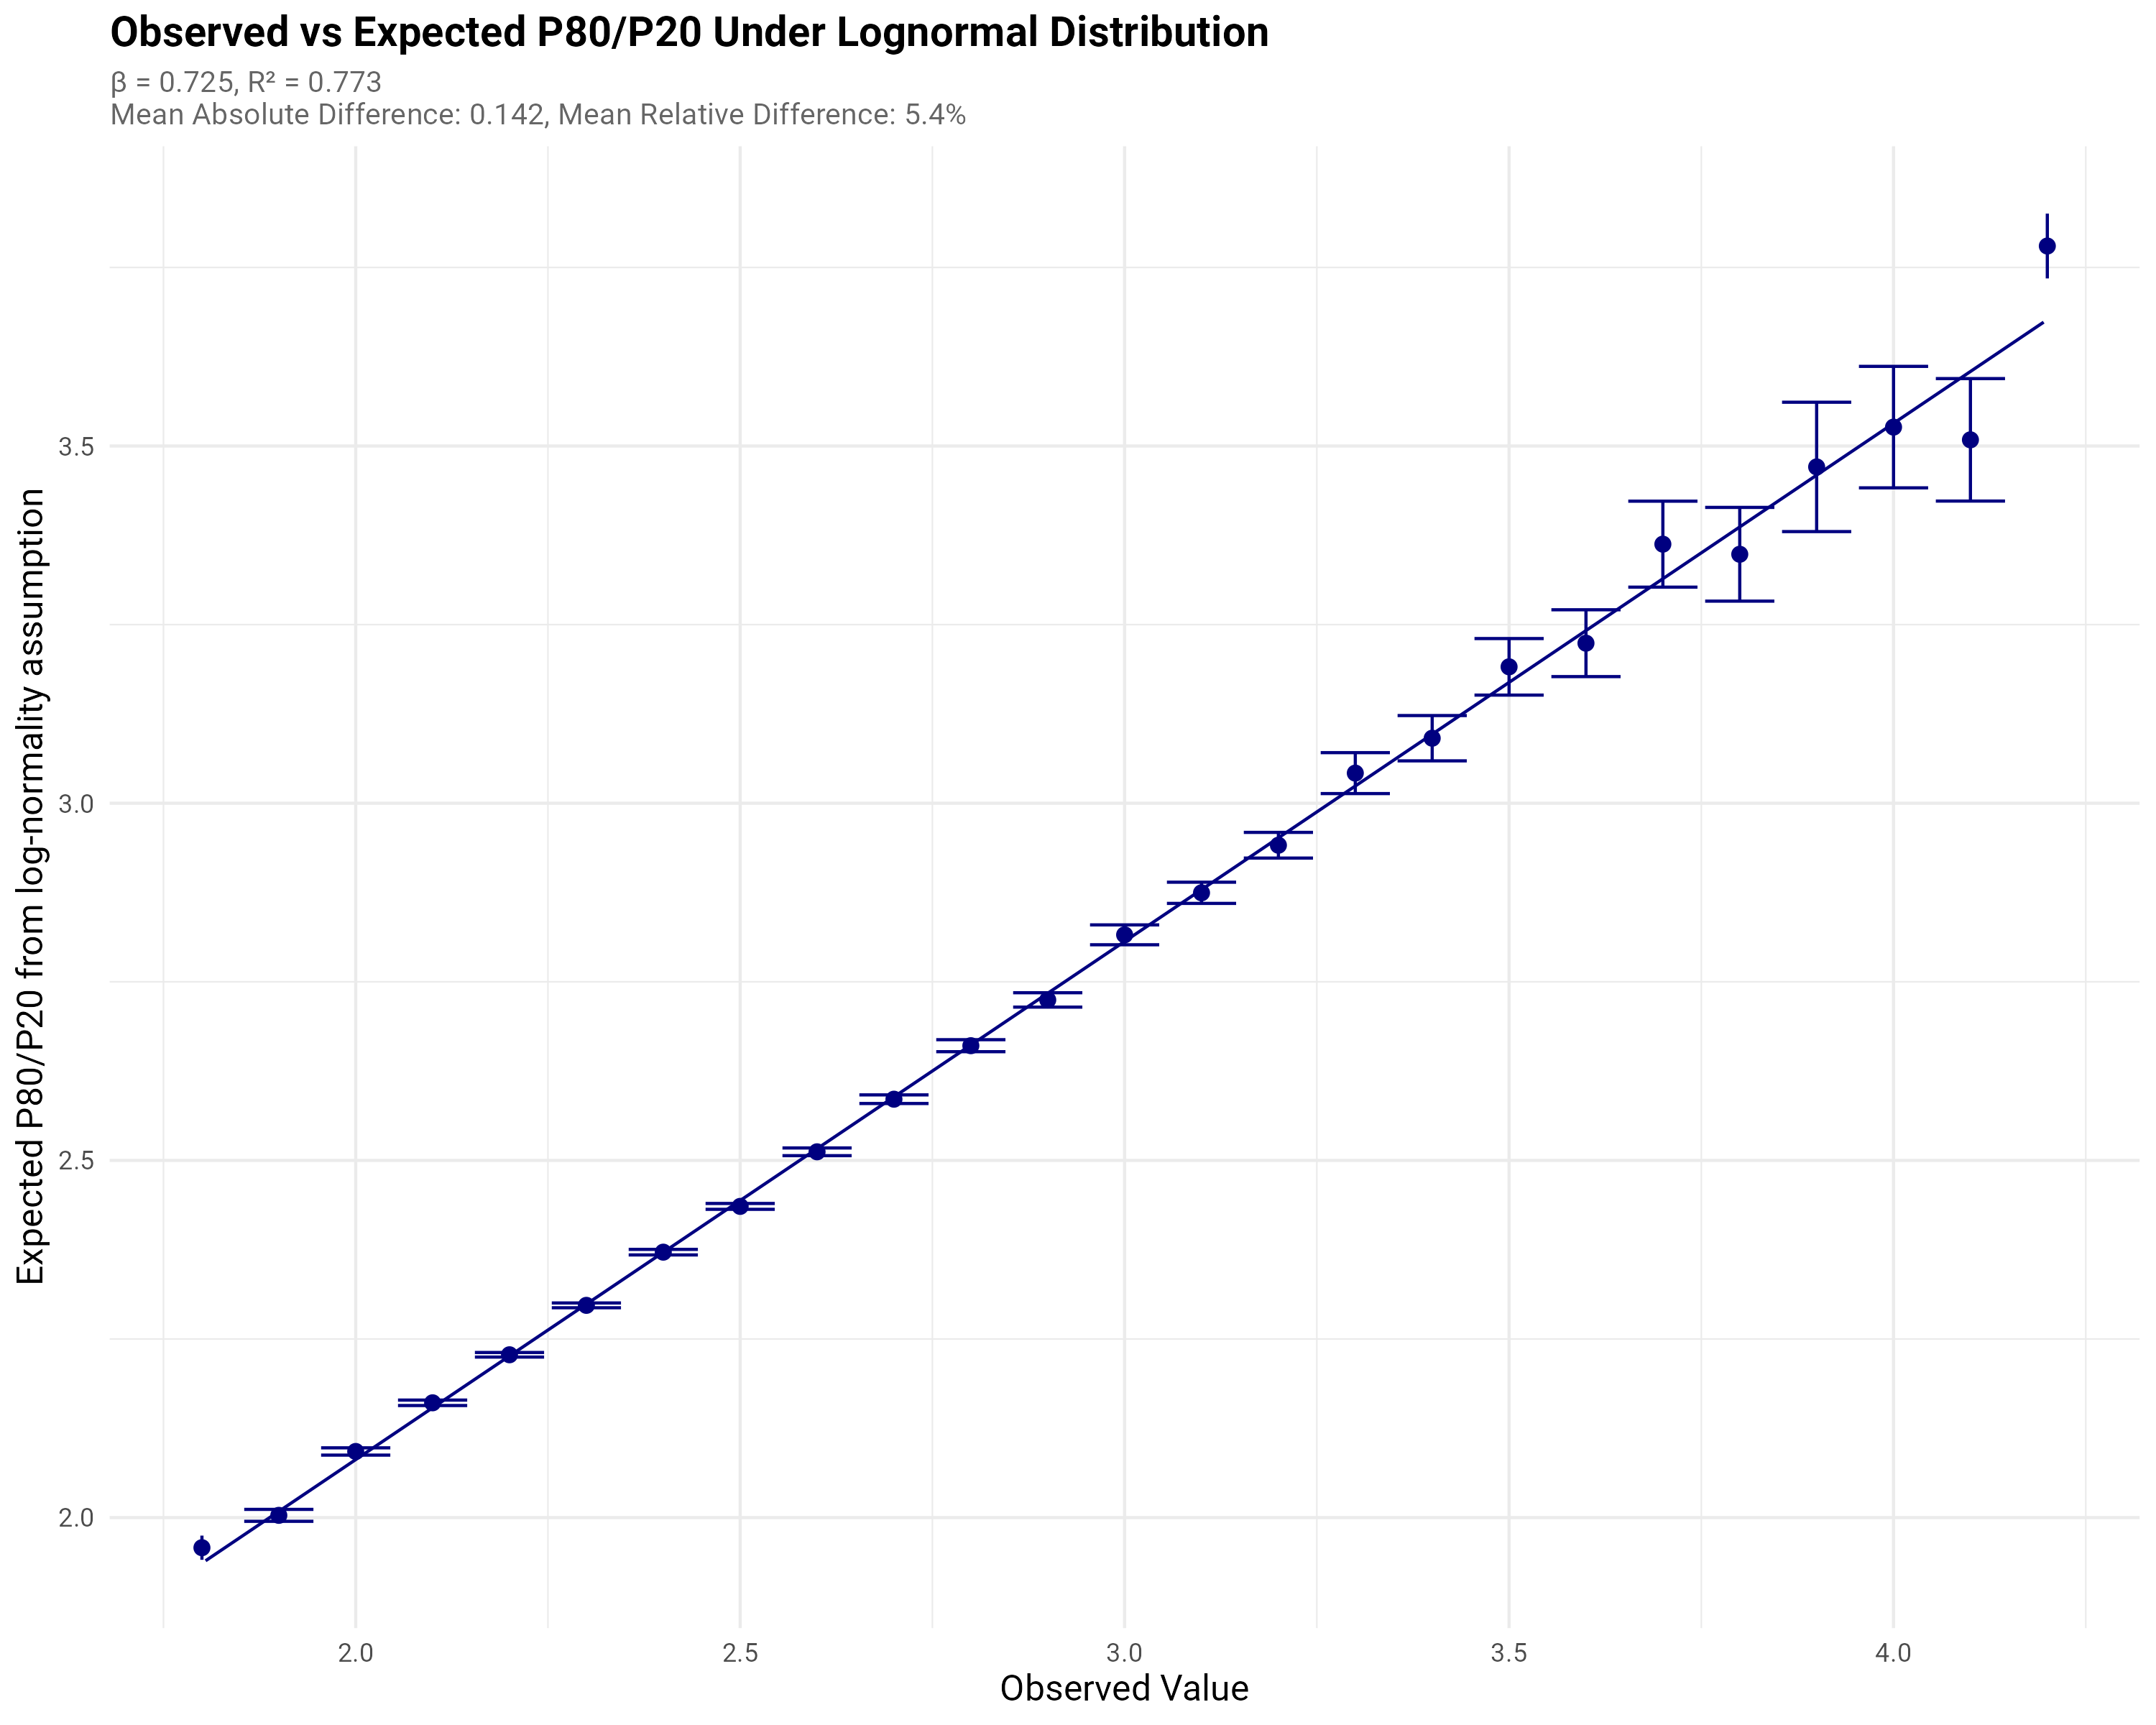
\includegraphics[width=0.85\textwidth]{output/binned_scatter_p80p20.png}
\end{center}
\begin{fignotes2}
\textbf{Notes:} This figure shows a binned scatter plot comparing observed P80/P20 ratios with predicted values under the log-normal assumption for each census tract. Source: Spanish Statistical Office and author's calculations.
\end{fignotes2}
\end{figure}

% \begin{figure}[H]
% \begin{center}
% \captionsetup{justification=centering}
% \caption{Estimated mixture vs. tract means}
% \label{fig:distributions}
% 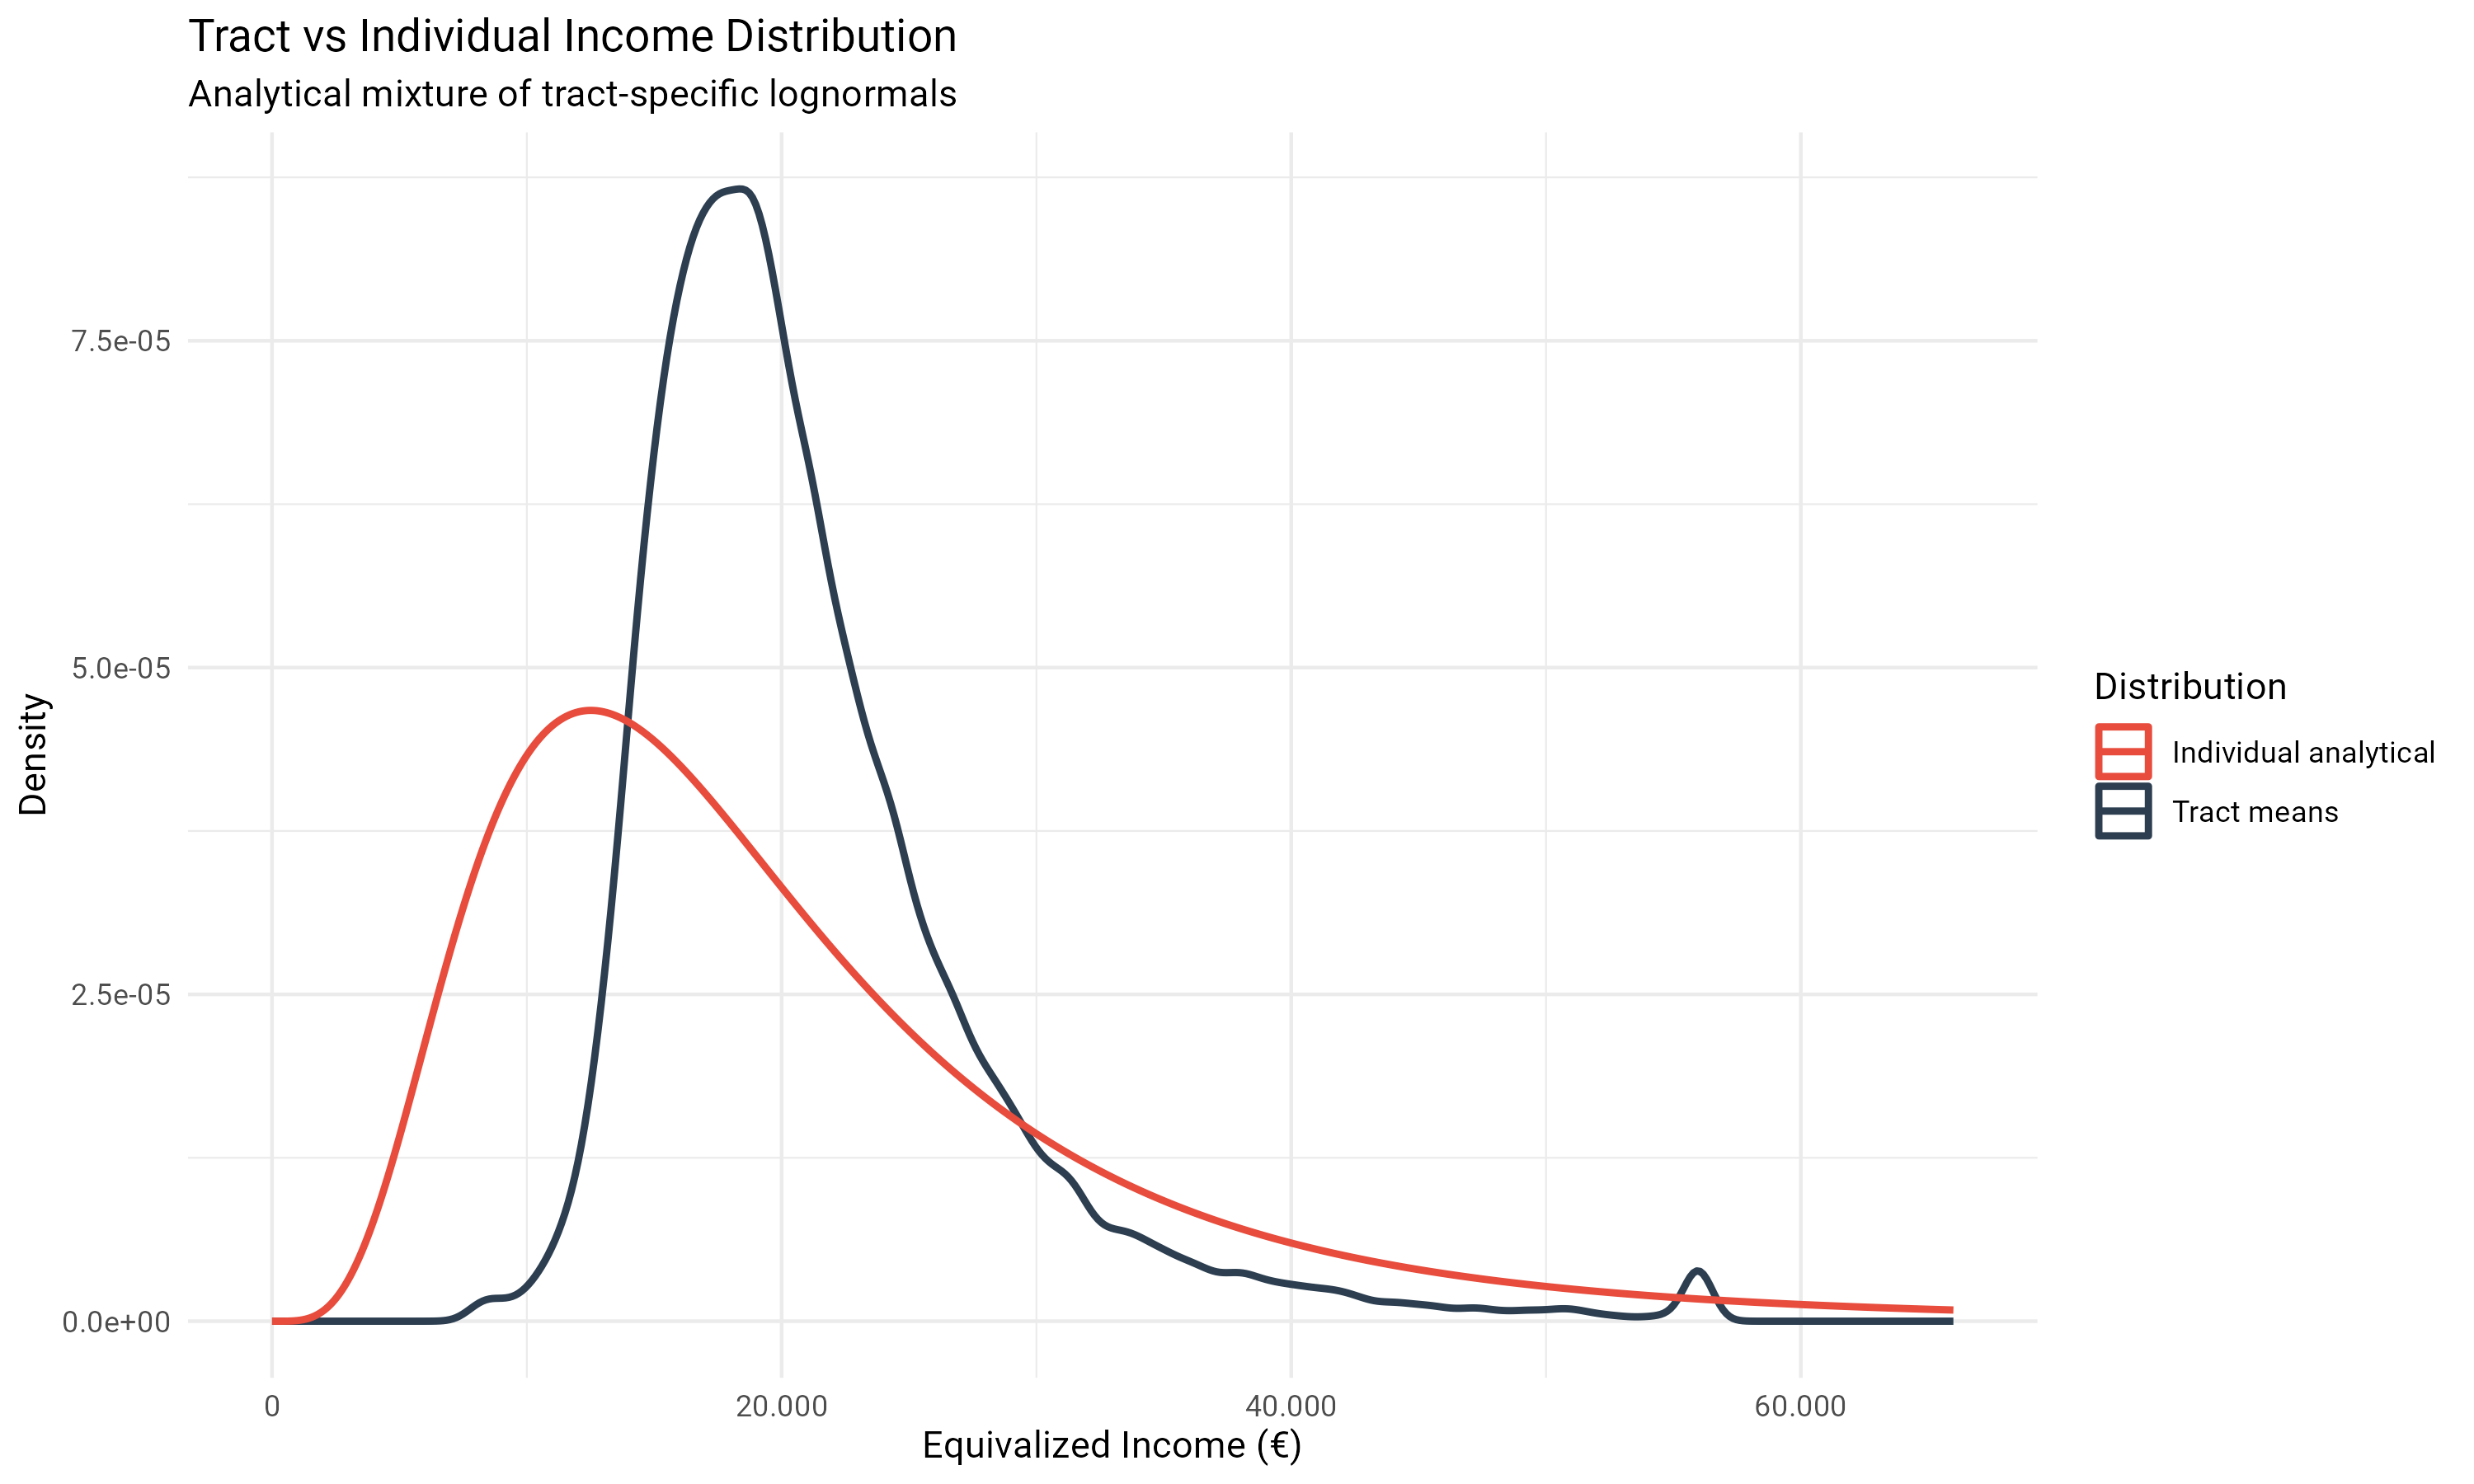
\includegraphics[width=0.7\textwidth]{output/tract_vs_individual_income_distribution.png}
% \end{center}
% \begin{fignotes2}
% \textbf{Notes:} This figure shows two approaches to approximating the individual income distribution: using tract means (in dark blue), where everyone within a tract is assumed to have the same income, and using a mixture of log-normals (in red) that incorporates within-tract inequality. The tract means distribution is calculated as a population-weighted kernel density of tract means. The mixture distribution is constructed using tract-specific log-normal distributions, where the parameters of each component are derived from observed tract means and Gini coefficients, and mixture weights correspond to tract population shares. Data refers to year 2022. Source: Spanish Statistical Office and author's calculations.
% \end{fignotes2}
% \end{figure}

A natural question arises: to what extent does exploiting local-level heterogeneity through a mixture of tract-specific distributions improve our measurement of the national income distribution compared to a simpler log-normal approximation? The comparison shown in Figure \ref{fig:dist2} reveals a striking finding: despite incorporating rich geographic variation in both average income and inequality metrics, the mixture distribution is remarkably similar to a single log-normal distribution fitted using only the national-level average income and Gini coefficient derived from household survey data (EU-SILC). This pattern aligns with previous evidence showing that log-normal densities approximate very well the empirical distribution of per capita income in large cross-country panels \citep{lopez2006normal}. In contexts where more granular data is not available, these results suggest that assuming log-normality at the national level might remain an accurate approximation for capturing the overall shape of the income distribution.

\begin{figure}[H]
\begin{center}
\captionsetup{justification=centering}
\caption{Estimated mixture vs. national log-normal}\label{fig:dist2}
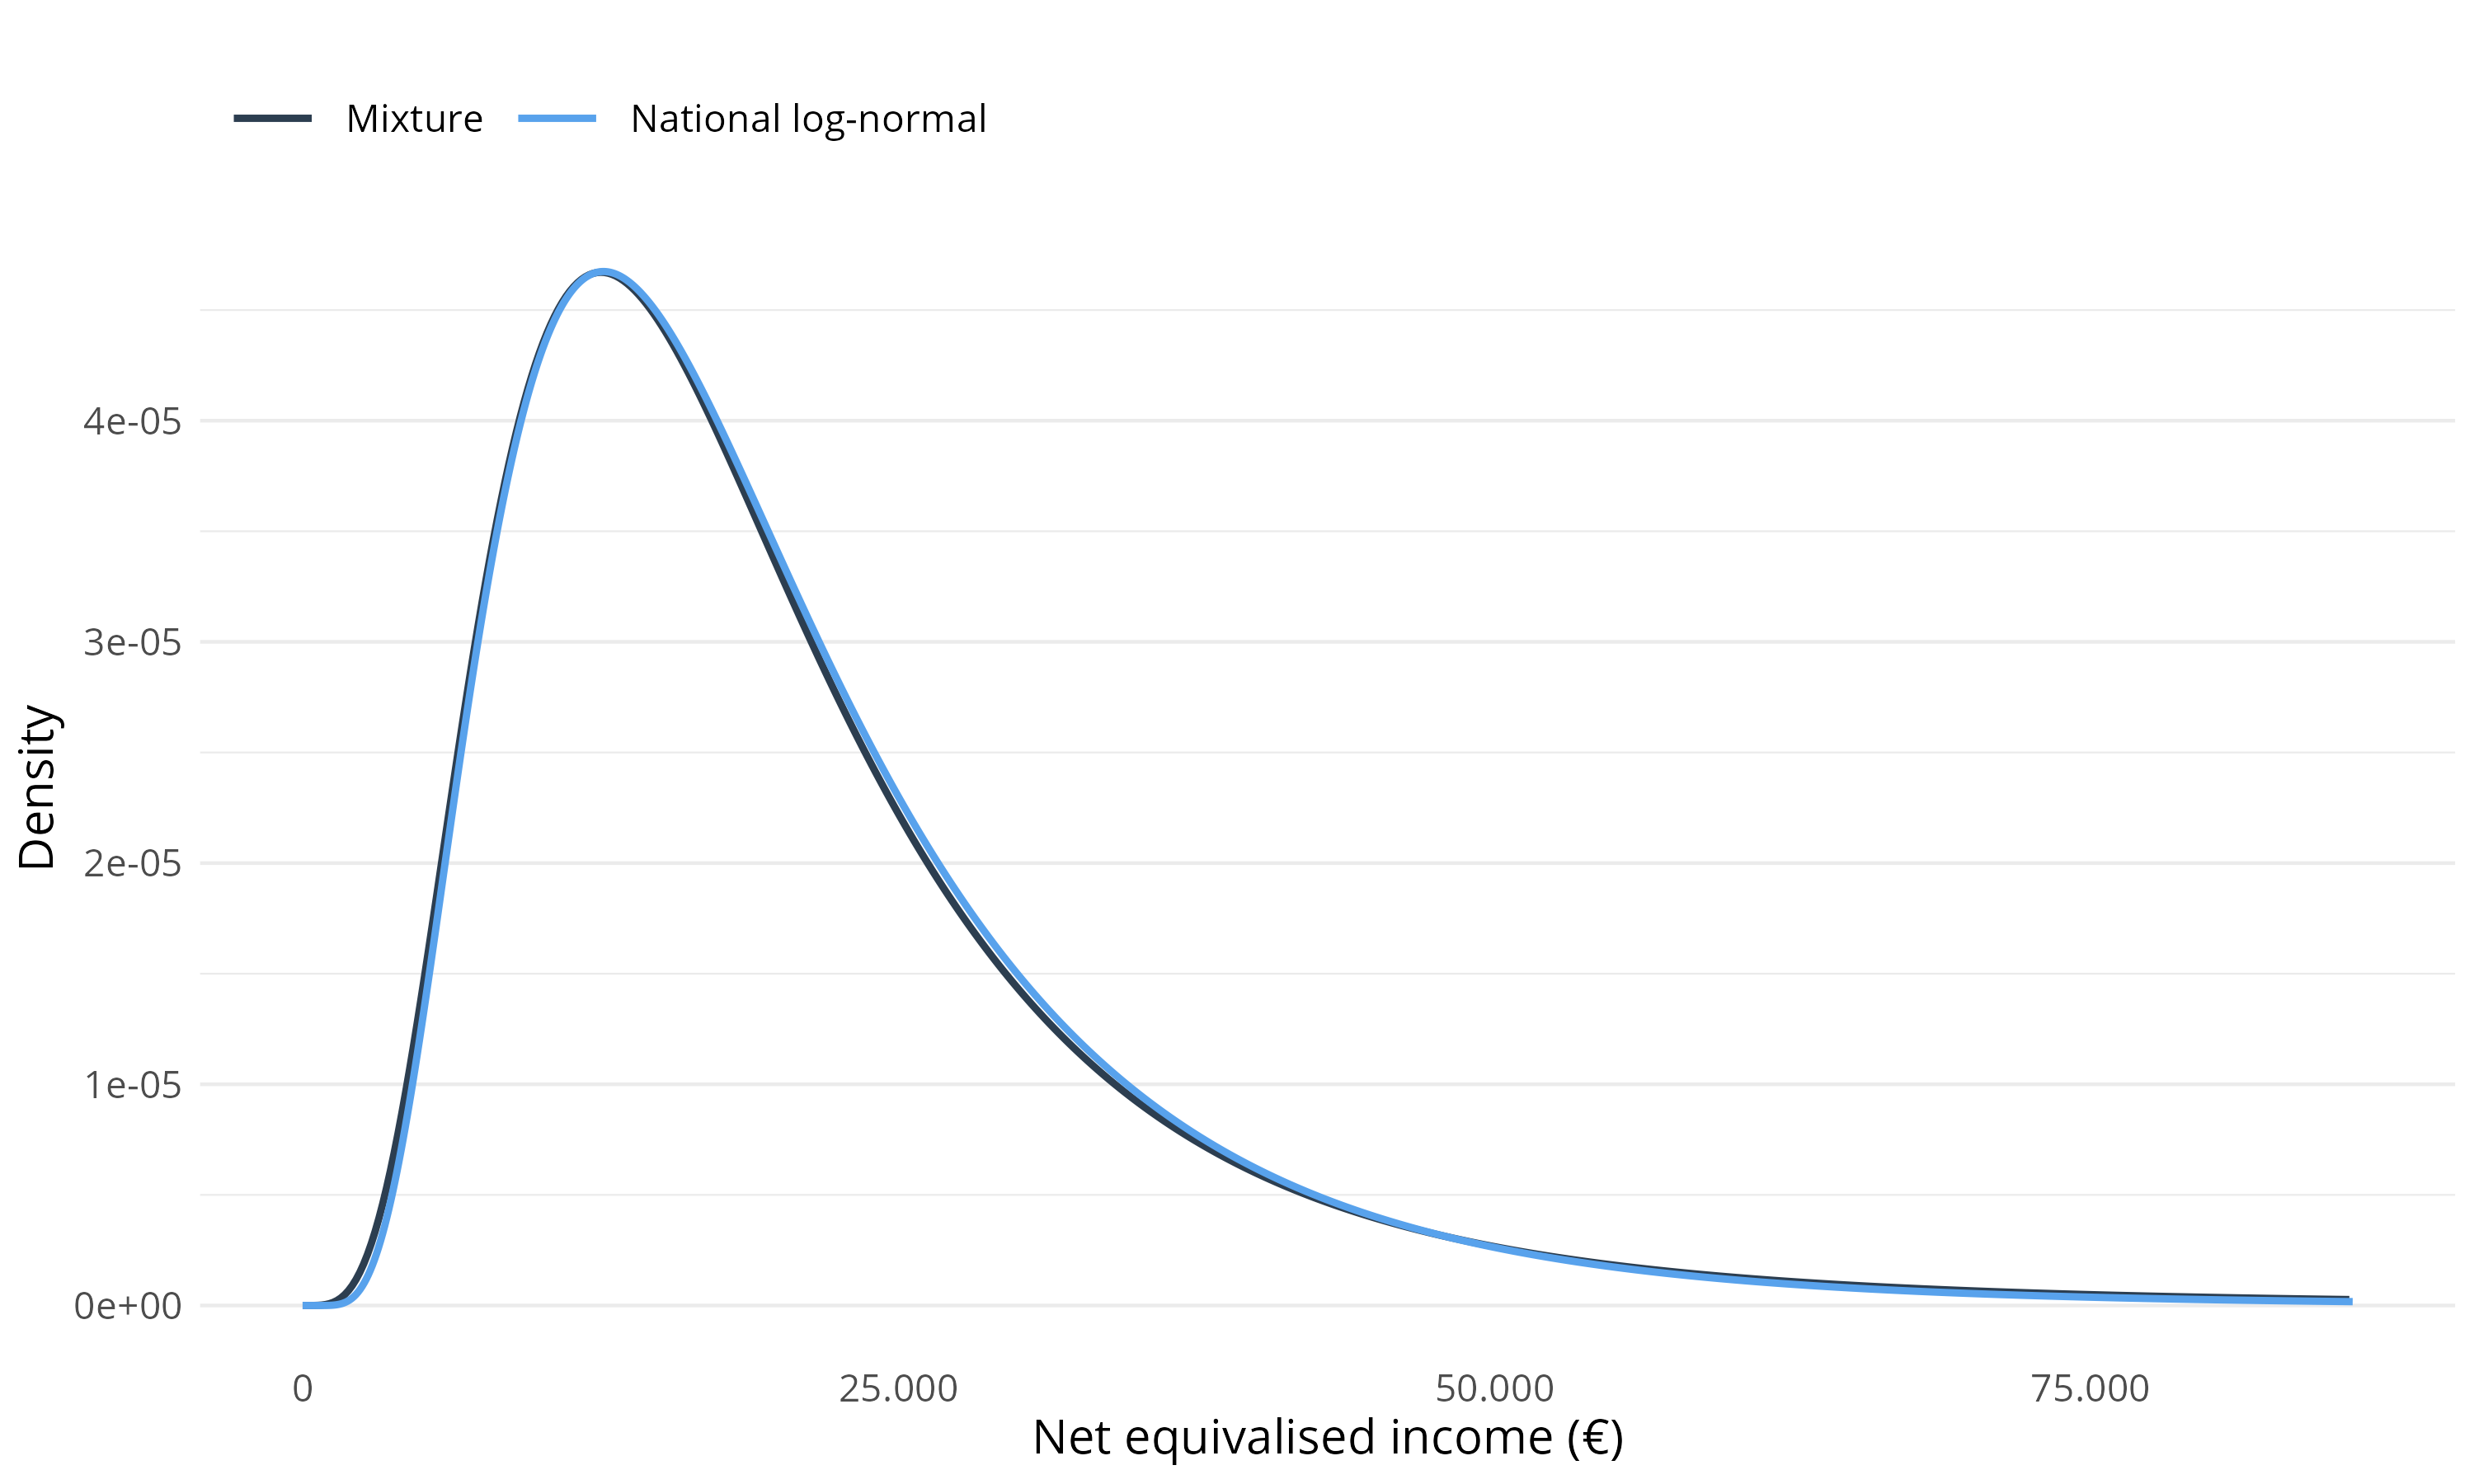
\includegraphics[width=0.85\textwidth]{output/tract_vs_national_income_distribution.png}
\end{center}
\begin{fignotes2}
\textbf{Notes:} This figure compares the income distribution derived from a mixture of tract-level log-normal distributions (navy) with a single national-level log-normal distribution (light blue). The mixture distribution is constructed using tract-specific log-normal distributions, where the parameters of each component are derived from observed tract means and Gini coefficients, and mixture weights correspond to tract population shares. The parameters for the national log-normal are given by the national-level mean income and Gini coefficient from EU-SILC 2023. Data refers to year 2022. Source: Spanish Statistical Office and author's calculations.
\end{fignotes2}
\end{figure}

To better understand this result, I examine the spatial structure of income inequality in Spain through a hierarchical variance decomposition exercise. Specifically, I decompose the total variance of log income within each autonomous community $c$  into components corresponding to different geographic levels as follows:

\begin{equation}\label{decomp}
\sigma^2_{c} = 
\underbrace{\sum_{j} w_j \sigma^2_{j}}_{\text{Within-tract}} + 
\underbrace{\sum_{k \in c} \sum_{j \in k} w_j \big( \mu_{j} - \mu_{k} \big)^2}_{\text{Between-tract}} + 
\underbrace{\sum_{p \in c} \sum_{k \in p} w_k \big( \mu_{k} - \mu_{p} \big)^2}_{\text{Between-municipality}} + 
\underbrace{\sum_{p \in c} w_p \big( \mu_{p} - \mu_{c} \big)^2}_{\text{Between-province}}
\end{equation}

where $\sigma^2_{j}$ is the variance of log income within each census tract $j$, $\mu_j$ is the mean log income in tract $j$, $\mu_k$ is the mean log income in municipality $k$, $\mu_p$ is the mean log income in province $p$, and  $\mu_{c}$ is the cross-tract mean log income within autonomous community $c$. Population weights for tracts, municipalities, and provinces, are denoted by $w_j, w_k, w_p$, respectively. The decomposition separates total income variation into four components: within-tract, between-tract (within municipalities), between-municipality (within provinces), and between-province variation. The within-tract component is calculated assuming log-normality within each tract.

Figure \ref{fig:variance_decomp} presents the results of this decomposition by autonomous community. The analysis reveals that within-tract variation accounts by far for the largest share of income inequality, representing between 85\% and 91\% of total variance within autonomous communities. This finding provides additional support for using tract-level distributional estimates as the fundamental building blocks for the aggregate distribution.\footnote{Notice that this does not contradict the earlier discussion on homogeneity in income-generating \textit{processes} within neighborhoods. The latter refers to the shared mechanisms (e.g., proportional shocks) influencing income trajectories within neighborhoods, but does not imply homogeneity in outcomes. Individual incomes can still vary significantly due to structural or stochastic factors.} A further 12\% is on average explained by between-tract, within-municipality differences. Income differences between municipalities and provinces contribute only marginally to overall income inequality.\footnote{Extending the decomposition analysis at the national level shows that between-community income disparities only account for 5\% of total variance.}

This predominance of within-tract variation provides intuition for why the mixture and single log-normal distributions are so similar. Since between-tract heterogeneity accounts for a relatively small share of total inequality, incorporating tract-level variation through a mixture approach adds limited value beyond a simple national-level approximation in the Spanish context.

\begin{figure}[H]
\begin{center}
\captionsetup{justification=centering}
\caption{Variance decomposition}
\label{fig:variance_decomp}
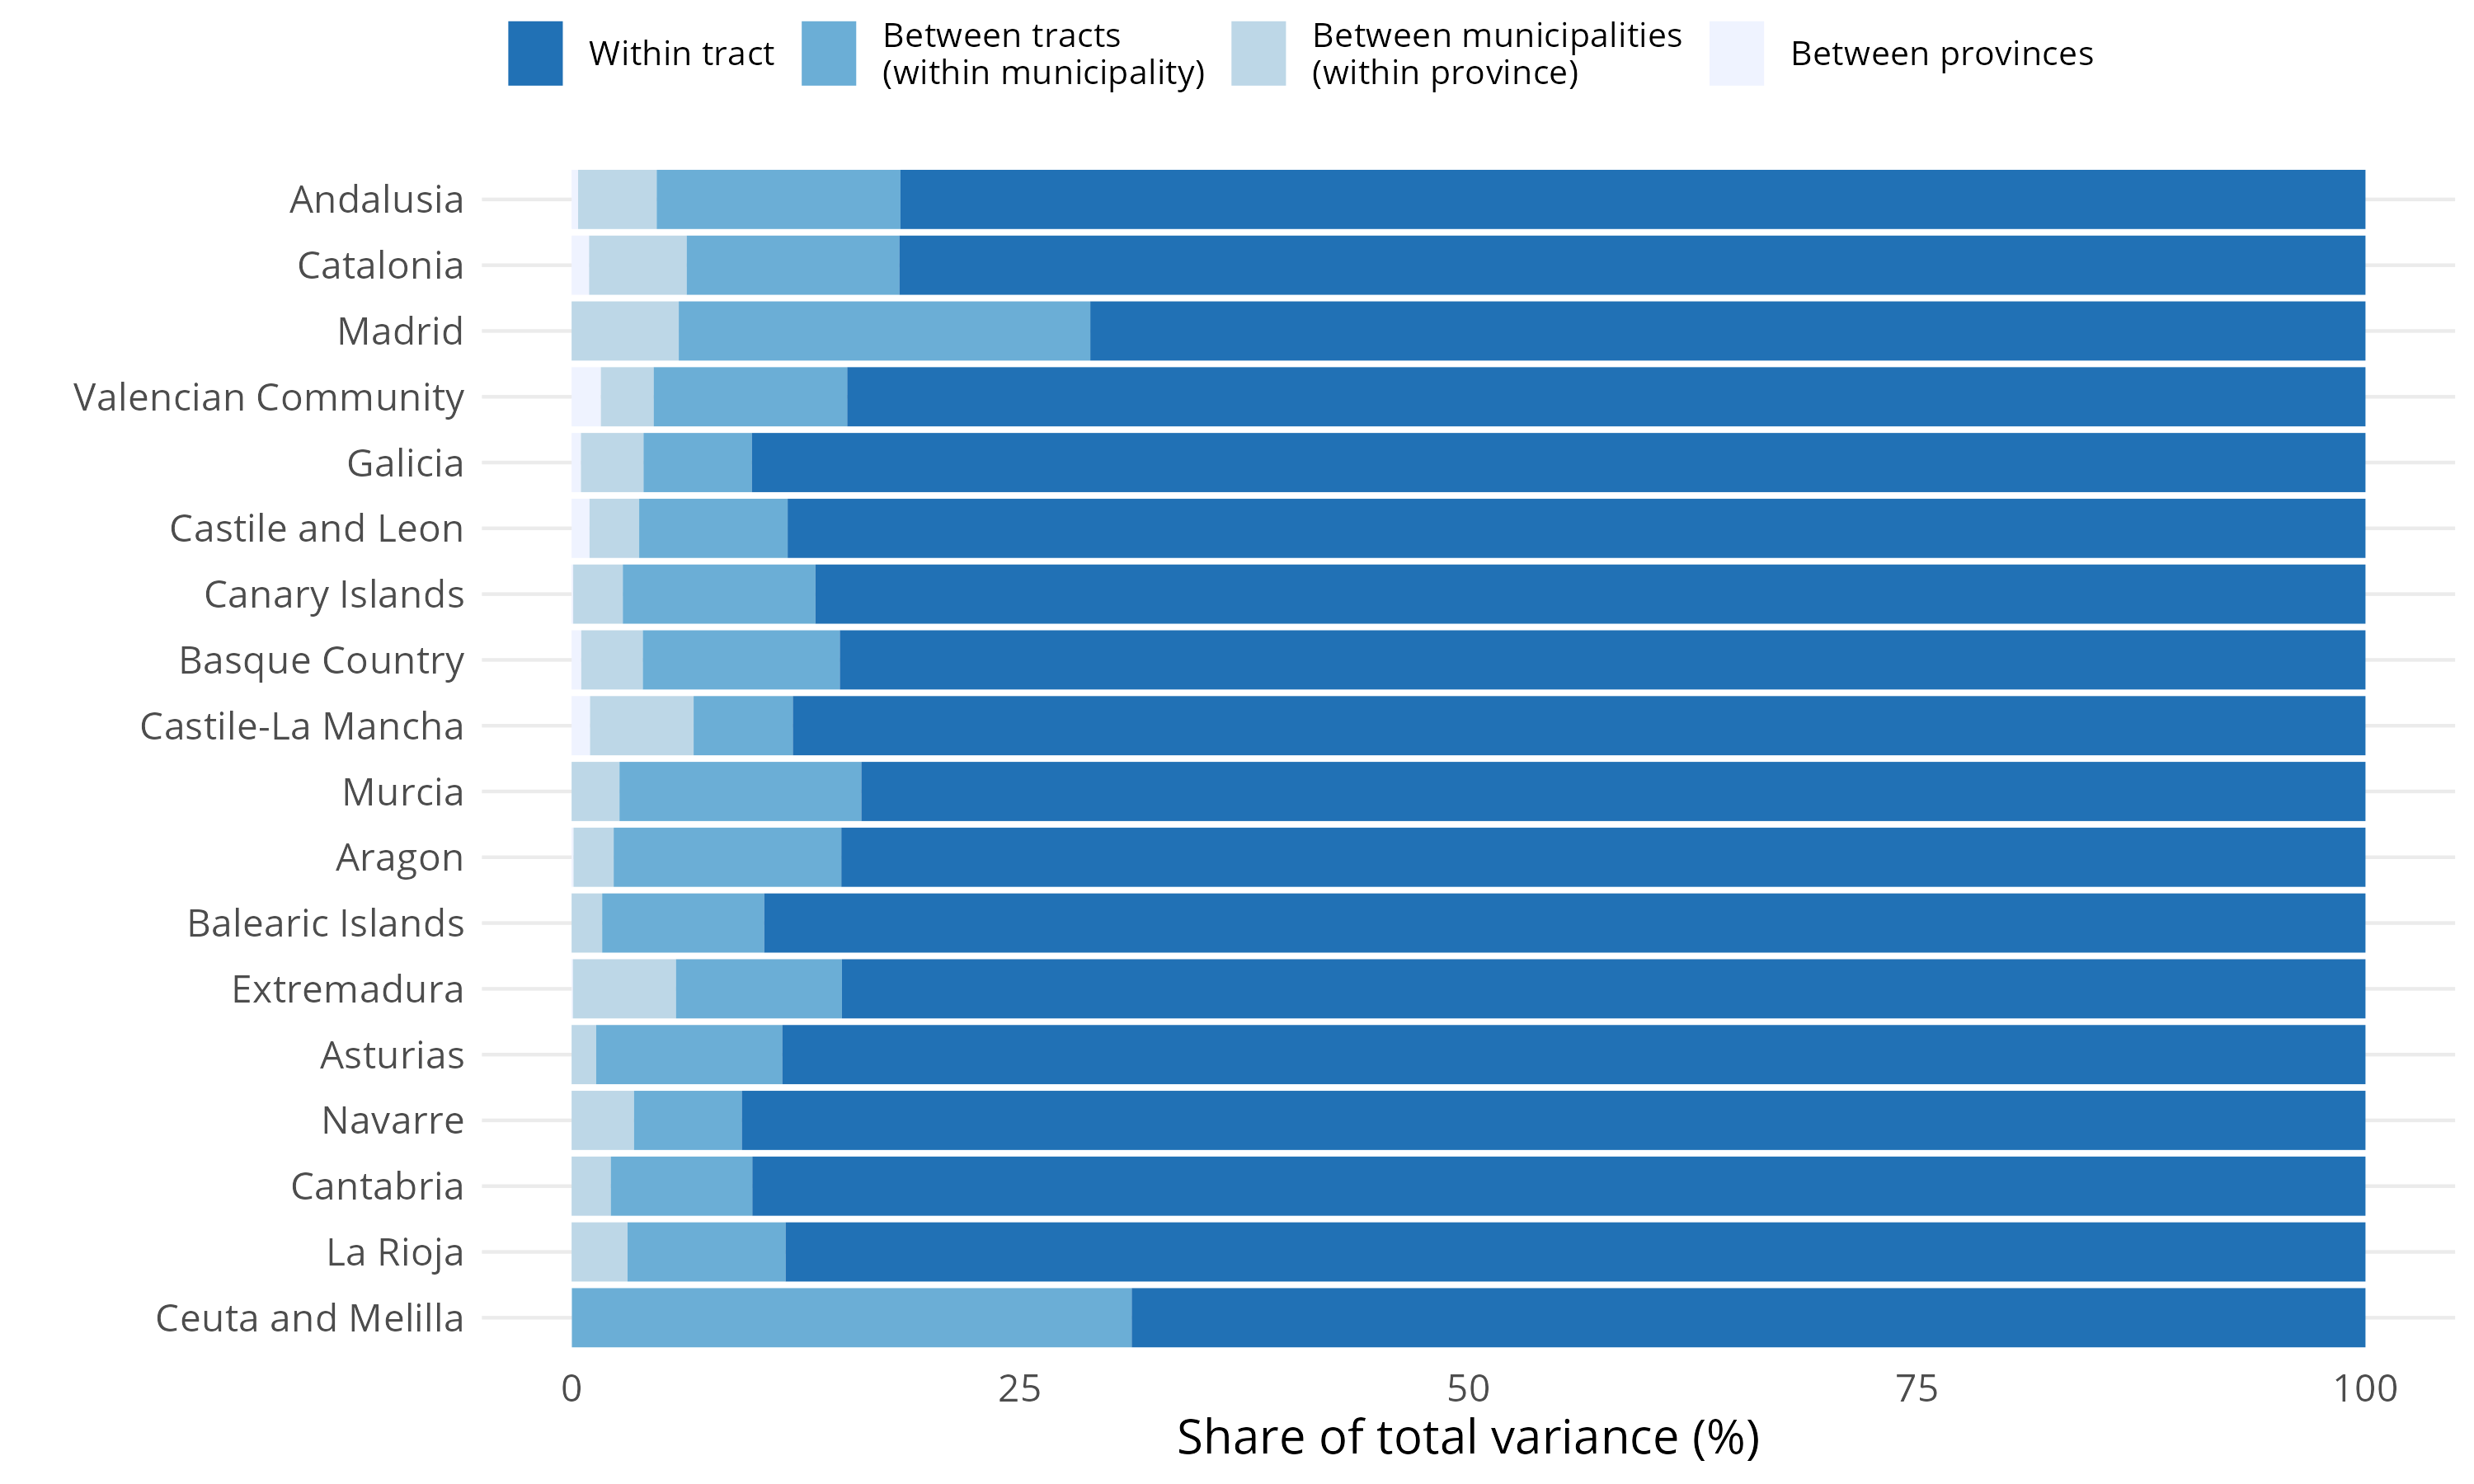
\includegraphics[width=0.85\textwidth]{output/variance_decomp.png}
\end{center}
\begin{fignotes2}
\textbf{Notes:} This figure shows the decomposition described in Equation \ref{decomp} whereby total variance in log income is broken down into four components: within-tract, between-tract (within municipality), between-municipality (within province), and between-province variation. The within-tract component is calculated assuming log-normality within tracts. Regions are ordered by total population. Source: Spanish Statistical Office and author's calculations.
\end{fignotes2}
\end{figure}

\section{Conclusion}\label{sec:conc}

This methodology note presents a simple framework for estimating income distributions in Spain, leveraging granular inequality metrics and administrative data at the census-tract level. Specifically, I model local income distributions as log-normal and derive national and regional distributions as population-weighted mixtures of tract-level estimates. Validation results show a high degree of accuracy, with predicted metrics closely matching observed distributional statistics across census tracts. Results from a hierarchical variance decomposition exercise show that within-tract variation explains the vast majority of income inequality in Spain.

% However, results also suggest that the improvement offered by the tract-level mixture relative to assuming log-normality at the national level is very limited, suggesting that the latter can still serve as a reasonable approximation to estimate aggregate distributions in the Spanish context. Results from a hierarchical variance decomposition exercise rationalize this finding by showing that within-tract variation explains the vast majority of income inequality in Spain, and hence accounting for between-tract heterogeneity adds relatively little information to the overall pattern of income inequality at the national level.

Looking ahead, the methodology offers opportunities for extension, such as explicitly addressing the deviations from log-normality at the tails of the distribution or adapting the framework for use in other countries with comparable data available. 

%Bibliography
\newpage
\singlespacing
\bibliographystyle{authordate3}
\bibliography{bib.bib}

\end{document}
